\documentclass[a4paper]{article}
\pagestyle{empty}
\usepackage{amssymb}
\usepackage{amsmath}
\usepackage{graphicx}
\usepackage{epstopdf}
\usepackage{color}
\usepackage[left=1.0in,top=1.0in,right=1.0in,bottom=2.5in]{geometry}
\setlength{\textwidth}{6.27in}
\setlength\topmargin{0.0in}
\setlength\headheight{0.5in}
%\setlength{\topmargin}{0.25in}
%\setlength\headheight{0.25in}

\usepackage{fancyhdr,lastpage}
\pagestyle{fancy}
\chead{Efficient Management of Coupled Multi-Physics Simulations Using SAGA-based Abstractions~\thepage~of \pageref{LastPage}}
\fancyhead[L]{}
\fancyhead[R]{}
\cfoot{A Hybrid CFD/MD Simulation on Multi-physical Fluid System using SAGA and BigJob, Page \thepage~of \pageref{LastPage}}


\newif\ifdraft
\drafttrue

\ifdraft
\newcommand{\fixme}[1]{ { \bf{ ***FIXME: #1 }} }
\newcommand{\jhanote}[1]{ {\textcolor{red} { ***Jha: #1 }}}
\newcommand{\jkimnote}[1]{ {\textcolor{blue} { ***JKim: #1 }}}
\else
\newcommand{\jhanote}[1]{}
\newcommand{\fixme}[1]{}
\fi

\begin{document}
\begin{center}


%%%%% TITLE %%%%%
\textbf {\large \bf Efficient Management of Coupled Multi-Physics Simulations
Using SAGA-based Abstractions: A Case Study of  Hybrid CFD/MD Simulation}
%\doublespacing
\vspace{14pt}

%%%%% AUTHORS %%%%%
\textbf {\normalsize \hspace{0.6 in} Joohyun Kim$^1$, Nayong Kim$^1$, Soon-Heum Ko$^1$, Dimitris Nikitopoulos$^2$  \newline Abhinav Thota$^1$, Shantenu Jha$^1*$ }

\vspace{12pt}

%%%%% AFFILIATIONS %%%%%
\normalsize { \hspace{0.6 in} $^1$Center for Computation and Technology, \newline Louisiana State University, Baton Rouge, LA 70803, USA}

\normalsize {\hspace{0.6 in} $^2$Mechanical Engineering Department, \newline Louisiana State University, Baton Rouge, LA 70803, USA}

\vspace{0.2in}
\footnotesize {\hspace{0.0 in} $^*$Corresponding Author sjha@cct.lsu.edu}


\vspace{12pt}

\end{center}

%%%%% MAIN TEXT %%%%%
Multi-Physics simulation techniques are being increasingly used to study physical phenomenon spanning time and length scales with varying level of details.  A hybrid CFD/MD approach~\cite{Nie:2004},~\cite{Yen:2007} is a simulation method which adopts the continuum hypothesis in capturing the macroscopic features of a flowfield\jkimnote{flow or "flow field" are not appropriate?} and resolves intermolecular effects on interfaces of different materials. CFD (Computational Fluid Dynamics) can accurately predict flow properties on conventional moderate/large size fluid domains, but is intrinsically impossible to reflect the characteristics of surrounding solid materials. MD (Molecular Dynamics) guarantees more accurate solution in that it also considers collision between fluid particles as well as interaction with solid particles, while its huge amount of computation time makes this method hard to solve a large scale system. An important challenge is solving a flowfield where viscous effect of solid boundary is dominant and the scale is sufficiently large in view of particle dynamics. These fluid systems can only be analyzed by solving particle interaction near the wall through molecular dynamics and applying a continuum approach on far field region. As is seen in Figure 1, the hybrid approach accurately describes strong interaction between solid elements and fluid particles near the wall and conducts efficient simulation in the far field follows the continuum approach.\jkimnote{in the last phrase, the subject of "follows the ..." is not clear due to the long sentence and sans the transition one such as comma}

In addition to the ``physics challenges'' of these Multi-Physics coupled simulations, there exist interesting ``computational challenges''. Probably the best known (and investigated) is the challenge of simulating large and complex systems, leading to simulations that require greater compuational resources -- often involving HPC resources, and no longer working on dedicated PCs. Another important challenge, especially for large-scale simulations is the need for effecient load-balancing, taking into account the individual simulation performance.

We have developed an {\it in-house} incompressible CFD code~\cite{Lee:2006} and LAMMPS MD simulation package (http://lammps.sandia.gov) \jhanote{Please put this in as a reference}, were used.\jkimnote{it is desirable to have similar two phrases. What about "and employed the in-house modified version of LAMMPS for MD"} We will report on the details of the communication mechanism employed elsewhere. Here we will focus on the challenges arising from running tightly-coupled simulations on production systems with batch-queues -- and thus it cannot be guaranteed that two separate jobs will execute concurrently.  As CFD and MD codes have frequent communications, (e.g., the CFD code conducts data exchange in every iteration) they need to run concurrently.  Thus, without explicit support for co-scheduling, it is unlikely that coupled CFD-MD simulations will run concurrently as inevitably the first job to run will have to wait for the other to follow.
% Users' account loss is inevitable in conventional queuing systems except when sufficient CPUs are idling, 
And even in cases where they can run concurrently, without explicit load-management/balancing support, there is likely to be inefficient utilization of compute resources due to load imbalance.  As the performance of each tool changes with computing resource and problem size, re-adjustment of allocated resources to each task according to their performance is required during the simulation. However, if the simulation have been submitted as independent jobs, changing CPU allocation to address these change is challenging. Thus, the best way in conventional job submission system would be to find a site with sufficient resource pool and submit two jobs with optimal number of processors according to the pre-test data on performance of each tool in that facility with the same problem size.

Given the lack of System or Service-level support to address the challenges outlined above, there is a need to address the solution at the user (application) level.  Here we outline our approach -- which is not-tied to a specific application set, is scalable and xtensible. SAGA (the Simple API for Grid Applications)~\cite{Jha:2008} is a high-level API which provides the basic functionality required to implement distributed applications in an infrastructure and middleware independent fashion.
% is designed to deal with distributed infrastructure explicitly and it supports application-level functionality/interface for distributed applications. 
SAGA enables the creation of higher-levels of abstractions, for example a contain-job and pilot-job, which is referred to as the BigJob abstraction~\cite{Jha:2009}.
-- which denotes a container task where a number of subtasks can run in pre-defined schedule with specified number of processors whether or not they are coupled.  Although the Container-Job/Pilot-Job concept is not novel {\it per se}, we believe this is the first documented utilization of these abstractions to perform coupled Multi-Physics simulations. Additionally, our approach employing a SAGA-based Pilot-Job is infrastructure neutral, unlike most other Pilot-Jobs.

The hybrid CFD/MD simulation consists of SAGA, SAGA glide-in framework and application framework (see Figure 1).  The BigJob Manager controls the BigJob submission, actual simulation of subtasks and promotes the re-launch of subtasks. The application framework is composed of two high-end simulation tools, application manager and load balancing module. By submitting a BigJob and specifying application components, the application manager enables the synchronous start of CFD and MD codes. When these two applications pause after producing checkpointing data and performance profile, the application manager can re-adjust processor allocation if required, to each subtask by the help of load balancing module and it eliminates the load imbalance between two application codes.  To achieve load balancing, we have implemented a simple load balancing function by the help of time checker in application codes. During the simulation, each application code returns its own simulation time. Assuming that each code has the ideal parallel performance, the load of each task would be the multiplication of their running time and number of processors used. Then, load balancing module re-adjusts resources inversely proportional to their presumed load. Considering every parallel code has different scalability, we can accomplish the load balance by a trial-and-error approach of above function.

The essential improvement of BigJob abstraction in this application lies in the removing the need\jkimnote{means" removing the need" without "the"?} for scheduling the two-components separately and in providing a single job-requirement to the queuing system. Additional efficiency is provided via application scenario specific load balancing modules.  We will contrast the specific scenarios -- from the {\it simple} Replica-Exchange, %to the In former replica exchange test, a bunch of small tasks with similar problem size were scheduled to run on the BigJob, leaving the requirement of load balancing among subjobs. On the other hand,
to the current scenario consisting of two tightly-coupled large-scale tasks and load balancing between two application components. % is the core of current simulation, as discussed above.
We will discuss architectural details of our solution, and provide performance data for three different BigJob scenarios to validate the usability and performance. In the first scenario, we will run one BigJob simulation which contains CFD and MD tasks and check the change of assigned number of processors to each task.  The same coupled simulation will be carried out by applying two BigJob simulations in the same computational resource to show the benefit of BigJob abstraction in acquiring maximal available computing resource and, the same test would be done on different heterogeneous systems to investigate the influence of multiple sites on the performance of BigJob. These test scenarios can be understood by the schematic on two BigJob submissions in Figure 1. When the first BigJob is allocated, two application codes run with predefined number of processors in each task. During the simulation, application framework changes the processor allocation according to load balancing function and would follow the optimal distribution. When the next BigJob is added to the running simulation, two BigJob resources are fully allotted to simulation codes and it repeats the same load balancing procedure.

\vspace{12pt}

%%%%% REFERENCES %%%%%
\begin{thebibliography}{99}
\bibitem{Nie:2004}
X. B. Nie, S. Y. Chen, W. N. E and M. O. Robbins,
\newblock "A Continuum and Molecular Dynamics Hybrid Method for Micro- and Nano-Fluid Flow,"
\newblock {\em J. Fluid Mech.}, 500, pp. 55-64, 2004

\bibitem{Yen:2007}
T. H. Yen, C. Y. Soong and P. Y. Tzeng,
\newblock "Hybrid Molecular Dynamics-Continuum Simulation for Nano/Mesoscale Channel Flow,"
\newblock {\em Microfluid Nanofluid}, 2007

\bibitem{Lee:2006}
Jung-Sang Lee, Chongam Kim and Kyu Hong Kim
\newblock "Design of Flapping Airfoil for Optimal Aerodynamic Performance in Low-Reynolds Number Flows,"
\newblock {\em AIAA Journal}, 2006

\bibitem{Jha:2009}
Shantenu Jha, Yaakoub El-Khamra, and Joohyun Kim,
\newblock "Developing Scientific Applications with Loosely-Coupled Sub-tasks,"
\newblock in {\em Computational Science - ICCS 2009}, G. Allen, J. Nabrzyski, E. Seidel, G.D. van Albada, J. Dongarra, P.M.A. Sloot (Eds.), Lecture Notes in Computer Science 5544, pp.641-650, 2009

\bibitem{Jha:2008}
A. Luckow, S. Jha, J. Kim, A. Merzky, and B. Schnor
\newblock Adaptive Replica-Exchange Simulations
\newblock {\em Royal Society Philosophical Transactions A} (to appear, 2009)
\end{thebibliography}

\vspace{12pt}

%%%%% FIGURES %%%%%

%================================================================
%  Add new figure (Figure 1) here
%================================================================
%\begin{figure}
%\centering
%\includegraphics[width=5.0in]{Image1.eps}
%\caption{CFD/MD Coupled Simulation on Channel Flow - Now Yet Included}
%\end{figure}
%================================================================

\begin{figure}
\centering
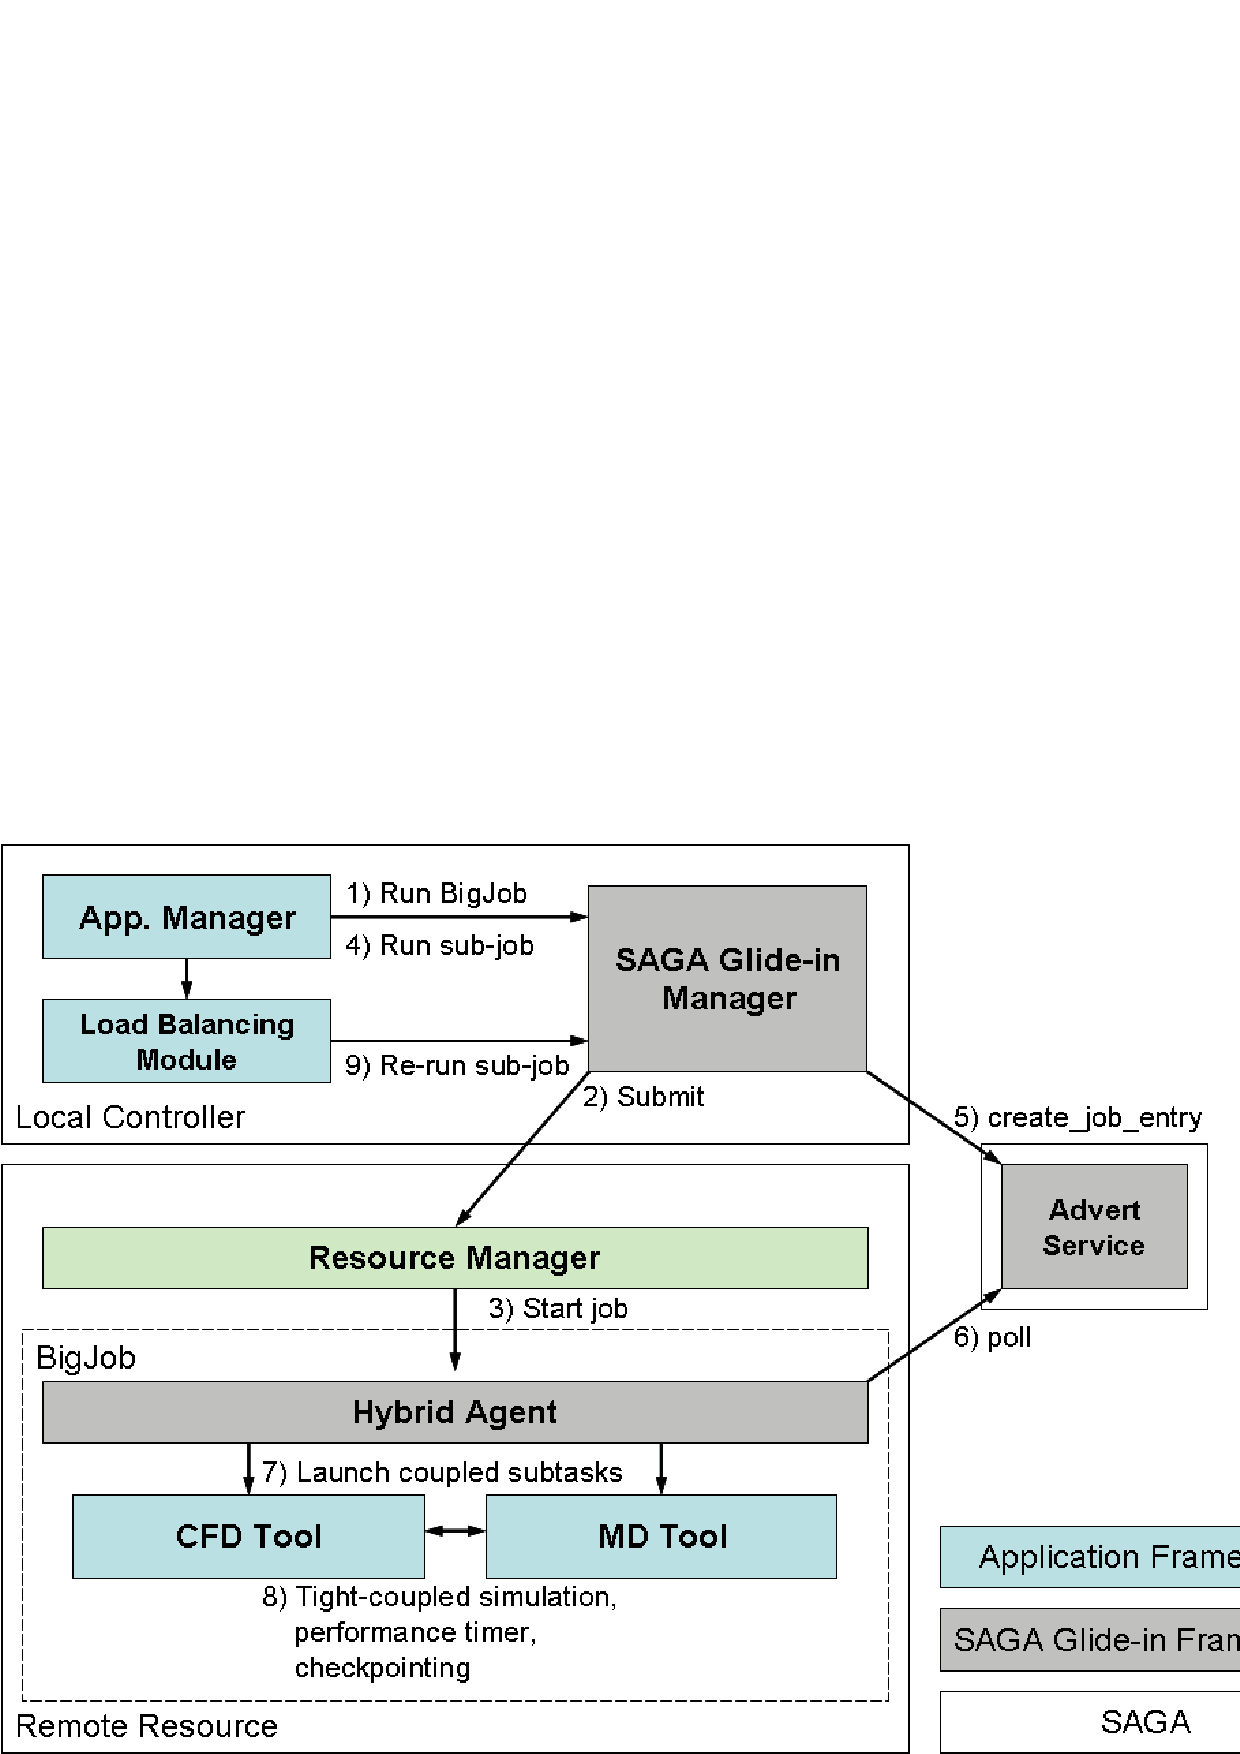
\includegraphics  [scale=0.33, angle=270]{Image2}
\caption{Architecture of the BigJob Abstraction for Hybrid CFD/MD Approach. \jhanote{Please change the ``SAGA Glide-In Manager'' to ``SAGA BigJob Manager''}}
\end{figure}

\begin{figure}
\centering
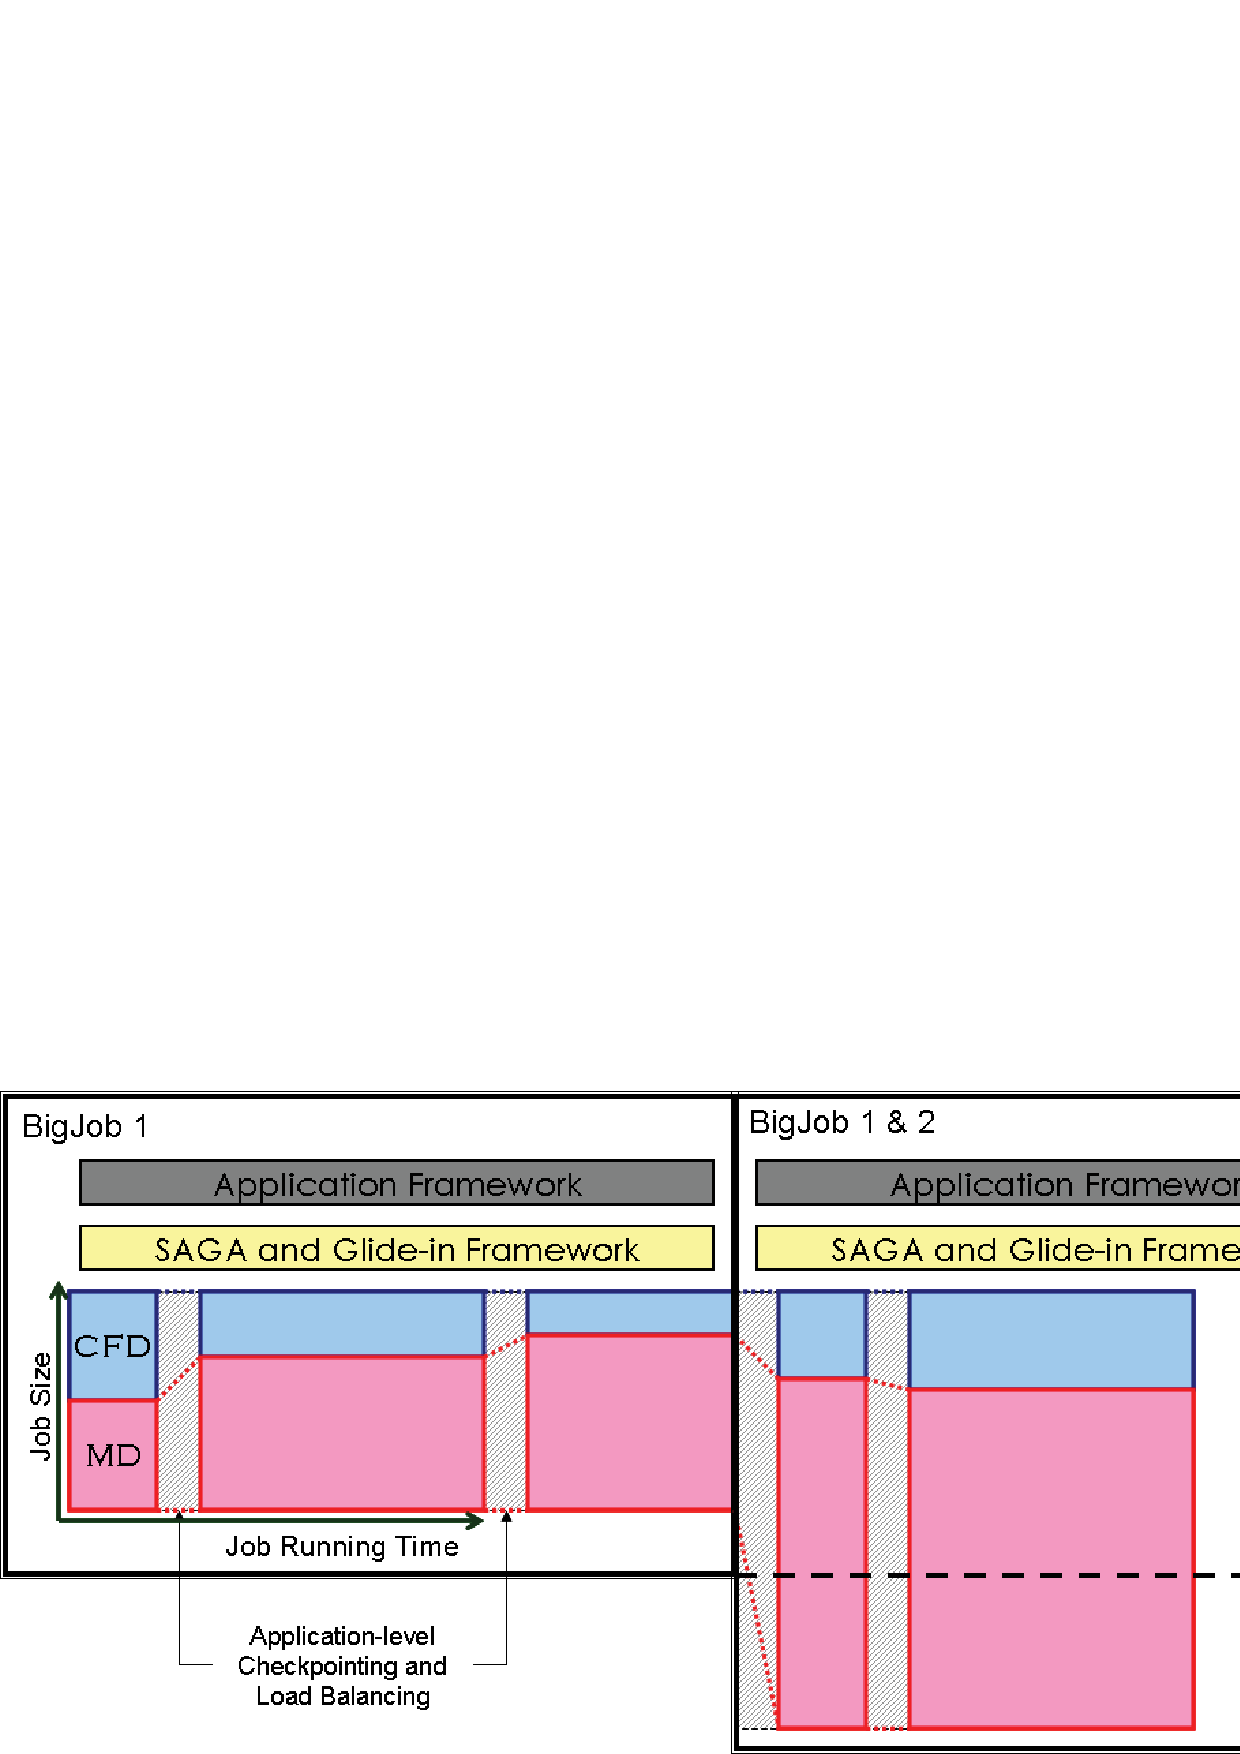
\includegraphics [scale=0.33, angle=270]{Image3}
\caption{The Scenario of Load-balanced Coupled Simulation with Two BigJob Abstraction.\jhanote{We have limit of 3 pages == 2 for text, 1 for figures. Please observer these constraints and adjust the size of these figures accordingly}}
\end{figure}

\noindent 

\end{document}


